\documentclass[10pt,a5paper]{book}
\usepackage[utf8]{inputenc}
\usepackage[english]{babel}
\usepackage{amsmath}
\usepackage{amsfonts}
\usepackage{amssymb}
\usepackage{geometry}
\usepackage{graphicx}
\usepackage{fancyhdr}
\usepackage{lipsum}
\usepackage{multirow}
\usepackage{verbatim}
\usepackage{xstring}
\usepackage{xcolor}

\pagestyle{fancy}

\definecolor{blue}{HTML}{115599}

\pagestyle{fancy}
\lhead{}
\rhead{Abstracts of ICCA10, August 4–9, 2014, Tartu, Estonia}

\newcommand{\abstract}[4]{
  \StrLeft{#1}{1}[\firstletter]
  \newpage
  \subsection*{\MakeUppercase{#3}}
  \subsubsection*{\scshape{#1 #2}}
  \addcontentsline{toc}{section}{
    \textit{\textbf{\firstletter. #2}}, #3
  }
  #4
}


\begin{document}

\begin{titlepage}

   \begin{center}
      \textcolor{blue}{ \Huge{ICCA10} }
      \textcolor{blue}{ \rule[1mm]{10.1cm}{0.7pt} } 
      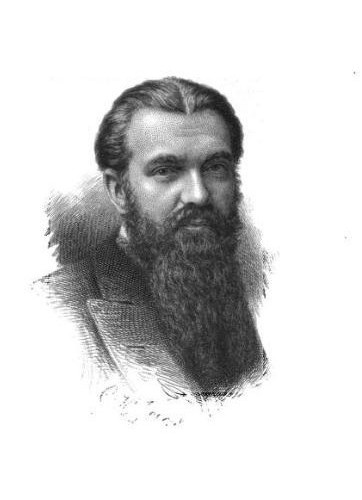
\includegraphics[scale=2]{clifford_large.jpg}\\      
      \textcolor{blue}{ \huge{\textbf{Book of Abstracts}} } \\
      \vspace{1cm}
      \textcolor{blue}{ \Large{$10^{\text{th}}$ International Conference on Clifford Algebras and their Applications in Mathematical Physics} } \\
      \vspace{1.4cm}
      \textcolor{blue}{ \small{\textbf{Tartu, Estonia \\ August 4–9, 2014}} }\\
   \end{center}
\end{titlepage}

\tableofcontents

\title{Abstracts of ICCA10, Tartu, 4–9 August 2014}

\newpage

\abstract{Arturas}{Acus}{Calculation of eigens with geometrical algebra rotors}{A practical  computational method to find the eigenvalues and
 eigenspinors of quantum mechanical Hamiltonian is presented. The
 method is based on reduction of the eigenvalue equation to
 geometrical algebra rotor equation, where the bivector in
 exponential rotor is constructed from two vectors, one is basis
 vector aligned with the quantization axis and the other comes from
 the rearrangement of the  Hamiltonian in geometric algebra form. A
 number of fully elaborated examples are presented in
 $\textit{Cl}_{3,0}$ algebra (monolayer graphene and spin in the
 quantum well) and $\textit{Cl}_{3,1}$ algebra (two coupled
 two-level atoms and bilayer graphene).}
\abstract{Daniel}{Alpay}{Schur analysis in the quaternionic setting”}{Schur analysis can be seen as a collection of problems pertaining to functions analytic and contractive in the open unit disk (Schur functions) in the setting of
 classical analysis, operator theory and signal processing. 
 Schur functions and Schur analysis have been extended to a number of settings, as diverse as compact Riemann surfaces and upper triangular operators. In the talk we
 begin with a brief survey of Schur analysis. We then consider the quaternionic setting, first in the framework of Fueter series, and then in the setting of slice-hyperholomorphic functions.
 
 }
\abstract{Swanhild}{Bernstein}{Riesz transforms in image processing and optics}{Riesz transforms play an essential role in image processing and optics. On one hand the are the building blocks of monogenic signals and on the other hand the also can be used as an substitue (in some sense) of derivatives in imaging and image processing. In this talk we would like to highlight the role of the Riesz transforms, fractional Riesz transforms and some fractional-type monogenic signals. These generalizations are based on quaternionic and Clifford calculus. }
\abstract{Kelvyn}{Brito}{The non-anticommutative supersymmetric Wess-Zumino model}{One introduces a deformation in the superspace through the anticommutation between parameters that are transformed from a Grassmann algebra into a Clifford algebra. After this, one analizes the deformation in the Wess-Zumino Lagrangian, searching for new interaction terms. }
\abstract{Isabel}{Cacao}{Quaternionic Zernike Spherical Polynomials}{The so-called Zernike polynomials (ZPs) were introduced by F. Zernike's Nobel prize in 1934 in connection to diffraction theory. They are constituted by the product of radial polynomials by a pair of trigonometric functions (sine and cosine) and they form a complete set of orthogonal polynomials over the unit circle. Since their appearance, a significant number of publications describing various applications of the ZPs have emerged, mainly in 
 optical engineering. They seem to be well-adapted to corneal
 surface modeling and they are commonly used
 to describe balanced aberrations. In this talk, we introduce the Zernike spherical
 polynomials within quaternionic analysis extending the classical two dimensional ZPs to dimension 3 or 4 in the quaternion algebra's framework. The representation of these
 functions in terms of spherical monogenics over the unit sphere are explicitly given,
 from which several recurrence formulae for faster computations can be
 derived. A summary of their fundamental properties and a second order
 differential equation are also discussed. }
\abstract{Rogerio}{Cavalcanti}{VSR symmetries in the DKP algebra: the interplay between Dirac and Elko spinor fields}{VSR symmetries are here naturally incorporated in the DKP algebra on the spin-0 and the spin-1 DKP sectors. 
 We show that the Elko (dark) spinor fields structure play an essential  role on accomplishing this aim, unravelling hidden symmetries on the bosonic DKP fields, which manifest 
 the intrinsic VSR symmetries of Elko fields. }
\abstract{Paula}{Cerejeiras}{tba}{later}
\abstract{Lander}{Cnudde}{Slice monogenic functions: algebraic approach and associated Clifford-Fourier transform}{In recent years, the study of slice monogenic functions has attracted more and more attention in the literature. In this talk, an extension of the well-known Dirac operator is defined which allows to establish the Lie superalgebra structure behind the theory of slice monogenic functions. According to this slice Dirac operator, an inner product is defined on a corresponding function space. Based on the polynomial null-solutions of this differential operator, an analogue to the classical Hermite polynomials is constructed. Together with the inner product, these polynomials allow for the construction of orthogonal and normalised Clifford-Hermite functions. Being analogues of the classical Hermite functions, they can be seen as eigenfunctions of a Clifford-Fourier transform. Corresponding to the Mehler formula in classical Fourier transform theory, a Mehler kernel is found for this Clifford-Fourier transform and its differential properties are investigated. The similarities between these properties and the differential properties of the classical Fourier kernel evoke a closer study of the solutions of the corresponding partial differential equation.}
\abstract{Fabrizio}{Colombo}{Some results on the F-functional calculus}{In this talk we introduce the two possible formulations of the F-functional calculus
  which are based on the Fueter-Sce mapping theorem in integral form.
  In the case of dimension $3$
 we show that there exists the F-resolvent equation
 and  we study the analogue of the Riesz projectors associated with this calculus.
 Moreover, we  show that it is possible to define this calculus
 also for $n$-tuples of unbounded operators and we obtain an integral representation formula analogous to
  the one of the Riesz-Dunford functional calculus for unbounded operators acting on a complex Banach space.}
\abstract{Oliver}{Conradt}{Projective Algebra $\Lambda_{n}$}{Projective algebra is defined as a double algebra $\Lambda_{n}(+,\ ,\wedge,\vee)$ together with an equivalence and a position relation. There is no metric present in pure projective geometry. The same holds for the $2^{n}$ dimensional algebra $\Lambda_{n}(+,\ ,\wedge,\vee)$. Geometric concepts such as primitive geometric forms, the principle of duality, cross ratio and projective mappings are introduced. Projective mappings $\Phi$ preserve the $\wedge$ and the $\vee$ product; one of both by definition, the second up to the factor $\det\Phi$. Binary indices for the basic elements of the projective algebra facilitate computations. The transition from projective to geometric Clifford algebra will be given.}
\abstract{Claude}{Daviau}{Gauge group of the standard model in $Cl_{5,1}$}{ABSTRACT. Describing a wave with spin 1/2, the Dirac equation is form invariant under  a group which is not the Lorentz group. This $SL(2,\mathbb{C})$ group is a subgroup of  $Cl_3^*=GL(2,\mathbb{C})$ which is the true group of form invariance of the Dirac equation. Firstly we use the $Cl_3$ algebra to read all features of the Dirac equation for a wave with spin 1/2. We extend this to electromagnetic laws. Next we use both the
$Cl_3$ algebra and the space-time algebra to get the gauge group of the electro-weak
interactions, first in the leptonic case, electron+neutrino, next in the quark 
case. The complete wave for all objects of the first generation uses two supplementary 
dimensions of space and the Clifford algebra
$Cl_{5,1}$. It is a function of the usual space-time with value into this enlarged
algebra. The gauge group is then enlarged into a $U(1)\times SU(2)\times SU(3)$ Lie group
in a way which gives automatically the insensitivity of electrons and 
neutrinos to strong interactions. This study gives new insights for many features of the
standard model. It explains also how to get three generations and four kinds of neutrinos.
We encounter not only two remarkable identities, we are able to explain several enigmas, like
the existence of the Planck constant or why the great unification based on $SU(5)$ could not be
successful. We consolidate both the standard model and the use of Clifford algebras as
the true mathematical frame of quantum physics. We present in concluding remarks a
simple solution to integrate together gravitation and quantum physics.
Then the only great domain of physics which remains to study is the electromagnetism with magnetic monopoles.}
\abstract{Hendrik}{De Bie}{The kernel of the Dunkl Dirac operator as a module for the Bannai-Ito algebra}{In this talk I will discuss how the CK or Cauchy-Kowalewska extension procedure can be developed for the Dunkl Dirac operator related to the reflection group $(Z_2)^m$. This will be used to construct an explicit basis for the kernel in dimension three, expressed in terms of Jacobi polynomials. In turn, by determining the symmetries of the Dunkl Dirac operator in dimension three, we obtain an unexpected connection with the Bannai-Ito algebra and with a scalar operator that also factorizes the Dunkl Laplacian. A detailed comparison will be given between the two approaches.}
\abstract{Hilde}{De Ridder}{Fueter's theorem in discrete Clifford analysis}{In 1935, R. Fueter described in his paper [1] a technique to obtain monogenic quaternionic functions, starting from a holomorphic function in the upper half of the complex plane. This classical result was later generalized to $\mathbb{R}_{0,m}$ for $m$ odd by Sce [2], for $m$ even by [3] and by Sommen in [4]: if $m$ is an odd positive integer and $P_k(\underline{x})$ is a homogeneous monogenic polynomial of degree $k$ in $\mathbb{R}^m$, then $\Delta_x^{k+\frac{m-1}{2}} \left[ \left( u(x_0, r) + \underline{\omega} \, v(x_0,r)\right) P_k(\underline{x}) \right] $ is also monogenic in $\widetilde{\Omega}$.
In this presentation, we consider a discretization of Sommen's result to the setting of (hermitean) discrete Clifford analysis in even dimension: starting from a discrete monogenic function in $\mathbb{Z}^2$, we will construct monogenic functions on $\mathbb{Z}^m$. [1] R. Fueter, Die funktionentheorie der Differentialgleichungen $\Delta u = 0$ und $\Delta \Delta u = 0$ mit vier variablen, Comm. Math. Helv. 7 (1935), pp. 307-330. [2] M. Sce, Osservazioni sulle serie di potenze nei moduli quadratici, Atti Accad. Naz. Lincei. Rend. Cl. Sci. Fis. Mat. Nat. (8) 23, 1957, pp. 220-225. [3] K. I. Kou and T. Qian and F. Sommen, Generalizations of Fueter's theorem, Methods Appl. Anal. 9 no. 2, 2002, pp. 273-289. [4] F. Sommen, On a generalization of Fueter's theorem, Z.Anal. Anwendungen 19 no.4, 2000, pp. 899-902.}
\abstract{Pierre-Philippe}{Dechant}{Platonic solids generate their four-dimensional analogues}{We show how regular convex 4-polytopes – the analogues of the Platonic solids in four dimensions – can be constructed from three-dimensional considerations concerning the Platonic solids alone. Via the Cartan–Dieudonne theorem, the reflective symmetries of the Platonic solids generate rotations. In a Clifford algebra framework, the space of spinors generating such three-dimensional rotations has a natural four-dimensional Euclidean structure. The spinors arising from the Platonic solids can thus in turn be interpreted as vertices in four-dimensional space, giving a simple construction of the four-dimensional polytopes 16-cell, 24-cell, the $F_4$ root system and the 600-cell. In particular, these polytopes have ‘mysterious’ symmetries, that are almost trivial when seen from the three-dimensional spinorial point of view. In fact, all these induced polytopes are also known to be root systems and thus generate rank-4 Coxeter groups, which can be shown to be a general property of the spinor construction. These considerations thus also apply to other root systems such as $A_1\oplus I_2(n)$ which induces $I_2(n)\oplus I_2(n)$, explaining the existence of the grand antiprism and the snub 24-cell, as well as their automorphism symmetries. These results are discussed in the wider mathematical context of Arnold’s trinities and the McKay correspondence. These results are thus a novel link between the geometries of three and four dimensions, with interesting potential applications on both sides of the correspondence, to real three-dimensional systems with polyhedral symmetries such as (quasi)crystals, viruses and carbon onions, as well as four-dimensional geometries arising for instance in Grand Unified Theories and String and M-theory.}
\abstract{Valeriy}{Dvoeglazov}{Energy-Momentum Tensor in Electromagnetic Theory and Gravitation from Relativistic Quantum Equations}{We analyze the problems of definitions of the energy-momentum tensors
in the electromagnetic theory and the general relativity. The 
Bargmann-Wigner formalism  has been used for higher spins. 
It is based on the Dirac equations for high-rank 4-spinors. We compare our 
results with those obtained by the group of Acad. Logunov 
and Prof. Khrapko. The conclusion is that it is possible to define the 
energy-momentum tensor compatible with the Noether theorem in any relativistic theory, in self-consistent ways. Different opinions presented in articles and books have been discussed. Possible methods of experimental verification
have been proposed.}
\abstract{Vladimir}{Dzhunushaliev}{Nonassociatuve generalization of supersymmetry }{We consider a nonassociative generalization of supersymmetry: supersymmetry generators as nonassociative ones are considered. Associators for the product of three and four multipliers are defined. It is shown that using a special choice of parameters the associator of the product of four supersymmetry generators is connected with the angular momentum operator. The connection of operators decomposition with the hidden variables theory and alternative quantum mechanics is discussed.}
\abstract{David}{Eelbode}{(1) Transvector algebras in Clifford analysis AND (2) Operator exponentials for the Clifford-Fourier transform (talk in ``Quaternion and Clifford Fourier Transforms and Wavelets")}{(1) The starting point for this talk is the observation that classical harmonic and Clifford analysis are related to the representation theory for the Lie algebra $\mathfrak{sl}(2)$ or its orthosymplectic refinement $\mathfrak{osp}(1,2)$. These objects appear quite naturally as the Howe dual for the spin group, which acts on the space of smooth functions on $\mathbb{R}^m$ with values in either the trivial or spinor representation. In recent years it has become clear that Clifford analysis techniques can also be used to study more complicated conformally invariant differential operators (as classified by Fegan in his seminal paper from 1976), which then act on functions on $\mathbb{R}^m$ with values in more complicated representations for the spin group. Despite the fact that the algebraic framework describing the Howe duality in several variables is well-understood, in terms of the symplectic Lie algebra $\mathfrak{sp}(2k)$ or its refinement $\mathfrak{osp}(1,2k)$, we believe that this is not the only algebra which appears naturally within the setting of higher spin analysis. The aim of the lecture therefore, is to introduce the so-called transvector algebras (which are related to Yangians, as introduced in the framework of the Yang-Baxter equation) and to explain how they show up in various aspects of higher dimensional analysis. (2) This paper deals with the construction of an exponential representation for the Clifford-Fourier transform defined on multi-vector signals. This is done using the Hamiltonian of the harmonic oscillator, and relies on the classical symmetries underlying harmonic and Clifford analysis on $\mathbb{R}^m$.}
\abstract{David}{Eelbode}{(1) Transvector algebras in Clifford analysis AND (2) Operator exponentials for the Clifford-Fourier transform (talk in ``Quaternion and Clifford Fourier Transforms and Wavelets")}{(1) The starting point for this talk is the observation that classical harmonic and Clifford analysis are related to the representation theory for the Lie algebra $\mathfrak{sl}(2)$ or its orthosymplectic refinement $\mathfrak{osp}(1,2)$. These objects appear quite naturally as the Howe dual for the spin group, which acts on the space of smooth functions on $\mathbb{R}^m$ with values in either the trivial or spinor representation. In recent years it has become clear that Clifford analysis techniques can also be used to study more complicated conformally invariant differential operators (as classified by Fegan in his seminal paper from 1976), which then act on functions on $\mathbb{R}^m$ with values in more complicated representations for the spin group. Despite the fact that the algebraic framework describing the Howe duality in several variables is well-understood, in terms of the symplectic Lie algebra $\mathfrak{sp}(2k)$ or its refinement $\mathfrak{osp}(1,2k)$, we believe that this is not the only algebra which appears naturally within the setting of higher spin analysis. The aim of the lecture therefore, is to introduce the so-called transvector algebras (which are related to Yangians, as introduced in the framework of the Yang-Baxter equation) and to explain how they show up in various aspects of higher dimensional analysis. (2) This paper deals with the construction of an exponential representation for the Clifford-Fourier transform defined on multi-vector signals. This is done using the Hamiltonian of the harmonic oscillator, and relies on the classical symmetries underlying harmonic and Clifford analysis on $\mathbb{R}^m$.}
\abstract{Cohl}{Furey}{Charge Quantization from a Number Operator}{In the early seventies, Gunaydin and Gursey discovered $SU_c(3)$ quark structure in the split octonions. Using their anti-commuting ladder operators, $\alpha_i$, we show a direct route to a new $U(1)$ generator. This $U(1)$ generator behaves like electric charge, thereby allowing us to further identify states behaving like the electron and neutrino. Our proposed electric charge turns out to be proportional to a number operator, consequently illuminating why it is quantized. Using only this trio of ladder operators, and their conjugates, we construct a pair of  minimal left ideals,  which is shown to transform under $SU_c(3)$ and $U_{em}(1)$ as does a full generation of the standard model.}
\abstract{Ramon}{Gonzalez Calvet}{HOW TO EXPLAIN AFFINE POINT GEOMETRY}{    Hermann Grassmann based his extension theory on Möbius’ barycentric calculus [1]. According to Grassmann, a line is the exterior product of two points, a plane is the exterior product of three points, and an extension having what we now call $n$ dimension is the exterior product of $n+1$ points [2]. Also, the exterior product of a line and a point is a plane, and the exterior product of two non-intersecting lines is the affine space. How should we explain this Grassmann’s point geometry to our pupils instead of the usual vector geometry? The algebraic way to teach it [3] is by using barycentric and homogeneous coordinates [4]. It will be shown that they have many advantages such as the natural introduction to projective geometry and duality which become trivial when they are understood by means of pencils of lines and sheaves of planes.
 
[1] A. F. Möbius, Der Barycentrische Calcul (Leipzig, 1827). Facsimile edition of Georg Olms Verlag (Hildesheim, 1976).
[2] H. Grassmann, Extension Theory (2000), in the series History of Mathematics vol. 19, American Mathematical Society and London Mathematical Society, p. 138. Translation of the 2nd edition of Die Ausdehnungslehre (Berlin, 1862) by Lloyd C. Kannenberg.
[3] R González Calvet, Treatise of Plane Geometry through Geometric Algebra, (Cerdanyola del Vallès, 2007) p. 43.
[4] R. González Calvet, El álgebra geométrica del espacio y tiempo, (2011-) http://www.xtec.cat/~rgonzal1/espacio.htm, p. 64.}
\abstract{Klaus}{Guerlebeck}{On $\psi$-hyperholomorphic functions}{ The theory of monogenic quaternion valued or Clifford algebra valued functions can be seen as refinement of harmonic analysis and as generalization of the complex function theory of holomorphic functions. We will follow in the talk the line of generalizing the complex function theory. Main topics are the characterization of hyperholomorphic functions by their geometrical mapping properties, the derivability and the construction of Taylor-type series expansions based on certain polynomial Appell systems. In a second step the relation of $\psi$-hyperholomorphic functions to harmonic functions will be studied in the non-trivial case of mappings from $\mathbb{R}^3\mapsto\mathbb{R}^3$ and an additive decomposition of harmonic functions in terms of $\psi$-hyperholomorphic functions will be proved. As applications we will discuss geometric properties of $\psi$-hyperholomorphic functions and the application to boundary value problems from linear elasticity.}
\abstract{Charles}{Gunn}{1) ``Geometric algebras for euclidean geometry" 2) ``Euclidean Plane Geometry using Projective Geometric Algebra"}{1) We discuss and compare existing GA models for doing euclidean geometry. We begin by clarifying a set of fundamental terms which carry conflicting meanings in the literature, including   $\mathbb{R}^{n}$, euclidean, homogeneous model, and duality. Equipped with these clarified concepts, we establish that the dual projectivized Clifford algebra $\mathbf{P(\mathbb{R}^*_{n,0,1})}$ deserves the title of standard homogeneous model of euclidean geometry (we also call it projective geometric algebra). We then turn to a comparison with the other main candidate for doing euclidean geometry, the conformal model. We establish that these two algebras exhibit the same formal feature set for doing euclidean geometry. We then compare them with respect to a set of practical criteria. 
2) On the basis of simple geometric exercises, we show how projective geometric algebra (PGA -- see talk 1)) can be used to teach euclidean plane geometry.  PGA contains the traditional vector algebra approach as a subset -- but contains many more unexpected delights that should please every lover of plane geometry, and provide a gentle introduction to those curious to get some practice using PGA.}
\abstract{Charles}{Gunn}{1) ``Geometric algebras for euclidean geometry" 2) ``Euclidean Plane Geometry using Projective Geometric Algebra"}{1) We discuss and compare existing GA models for doing euclidean geometry. We begin by clarifying a set of fundamental terms which carry conflicting meanings in the literature, including   $\mathbb{R}^{n}$, euclidean, homogeneous model, and duality. Equipped with these clarified concepts, we establish that the dual projectivized Clifford algebra $\mathbf{P(\mathbb{R}^*_{n,0,1})}$ deserves the title of standard homogeneous model of euclidean geometry (we also call it projective geometric algebra). We then turn to a comparison with the other main candidate for doing euclidean geometry, the conformal model. 
 We establish that these two algebras exhibit the same formal feature set for doing euclidean geometry. We then compare them with respect to a set of practical criteria. 
 2) On the basis of simple geometric exercises, we show how projective geometric algebra (PGA -- see talk 1)) can be used to teach euclidean plane geometry.  PGA contains the traditional vector algebra approach as a subset -- but contains many more unexpected delights that should please every lover of plane geometry, and provide a gentle introduction to those curious to get some practice using PGA.
 }
\abstract{Jacques}{Helmstetter}{Conformal Groups and Vahlen Matrices}{This article recalls some facts about the conformal group 
 Conf(V,Q) of a quadratic space (V,Q); in particular there is 
 a surjective group morphism O(V',Q')--->Conf(V,Q), where
 (V',Q') is the orthogonal sum of (V,Q) and a hyperbolic
 plane; its kernel is a group of order two. Then it explains 
 how the elements of O(V',Q') and Conf(V,Q) can be represented 
 by Vahlen matrices. And finally, it recalls some properties 
 of Vahlen matrices.}
\abstract{David}{Hestenes}{Electrodynamics of Electrons and Brains}{Maxwell’s equations for material media are formulated in terms of Geometric Algebra and related to differential forms. It will be argued that these equations are completely general and applicable to all phenomena in the Universe at all scales. Topological and metrical aspects of electromagnetic fields will be clearly distinguished, and their sources will be attributed to topological defects in a universal vacuum. Explicit forms for vacuum defects characterizing electron charge and spin will be given, and their generalization to all elementary particles will be discussed. Finally, application to understanding electromagnetic functioning of the brain will be discussed. }
\abstract{David}{Hestenes}{Electrodynamics of Electrons and Brains}{Maxwell’s equations for material media are formulated in terms of Geometric Algebra and related to differential forms. It will be argued that these equations are completely general and applicable to all phenomena in the Universe at all scales. Topological and metrical aspects of electromagnetic fields will be clearly distinguished, and their sources will be attributed to topological defects in a universal vacuum. Explicit forms for vacuum defects characterizing electron charge and spin will be given, and their generalization to all elementary particles will be discussed. Finally, application to understanding electromagnetic functioning of the brain will be discussed. }
\abstract{Eckhard}{Hitzer}{Quaternion Domain Fourier Transformation}{So far quaternion Fourier transforms have been mainly defined over $\mathbb{R}^2$ as signal domain space. But it seems natural to define a quaternion Fourier transform for quaternion valued signals over \textit{quaternion domains}. Such signals may e.g. represent vector fields in space and time. The quaternion domain Fourier transform thus developed may also be useful for solving quaternion partial differential equations or functional equations, three-dimensional time-dependent color field (space color video) processing, and in crystallography. We define the \textit{quaternion domain Fourier transform} and analyze its \textit{main properties}, including quaternion dilation, modulation and shift properties, Plancherel and Parseval identities, covariance under orthogonal transformations, transformations of coordinate polynomials and differential operator polynomials, transformations of derivative and Dirac derivative operators, as well as signal width related to band width uncertainty relationships.}
\abstract{Uwe}{Kaehler}{Fractional Clifford Analysis}{later}
\abstract{Igor}{Kanatchikov}{1) Precanonical quantization, quantum gravity and Clifford analysis (General session) / 2) On the structure of Standard Model from the point of view of precanonical quantization (in ``Geometric Algebra and Calculus in the Standard Model of Particle Physics")}{1) I will outline the precanonical approach to field quantization which leads to a generalization of quantum theoretic formalism were the space-time Clifford algebra 
 replaces the complex numbers in quantum mechanics: both the wave functions and operators are Clifford-valued. The approach also leads to a Dirac-like generalization of the Schroedinger equation with the mass term replace by the De Donder-Weyl Hamiltonian operator.  This formulation leads to an interesting class of problems which can be studied using the techniques of Clifford analysis. I will also discuss  how the precanonical approach leads to a nonperturbative quantization of  gravity where the quantum geometry is described by Clifford-valued transition amplitudes between different values of spin connection at different points. I show that the fundamental equation which describes the quantum geometry in this approach is a Clifford-algebraic matrix multi-variable generalization of the confluent hypergeometric equation. Thus the needs of quantum gravity call for a  study of generalizations of hypergeometric functions within the Clifford analysis.
 2) The approach of precanonical quantization of fields leads to a generalization of quantum theoretic formalism from mechanics to field theory. where the space-time Clifford algebra (which arises from quantization of differential forms) plays as important role as the complex numbers in quantum mechanics do. In this approach the space-time variables are treated on the equal footing and they play a role of the
 multidimensional analogue of the time parameter in quantum mechanics. I briefly discuss  the relation between precanonical quantization and the standard QFT in the functional Schroedinger representation and few interesting consequences of the application of precanonical quantization in the context of perturbative QFT (an application to quantum gravity will be discussed in the talk at the general session).  I also demonstrate that precanonical quantization of fermions naturally leads to the restriction of the number of fermionic fields which we can be incorporated into the (precanonically quantized) theory simultaneously in the way compatible with the standard functional Schroedinger representation. The number of fermions can not exceed the ability of the most general Clifford number on the space-time to embed the fermions in a linear way. This fact may have consequences for our understanding of the origin of symmetries of the Standard Model, as the latter should be related to the linear automorphisms of the space-time Clifford algebra and the dimensionality of the space-time, and also shed light on the possible nature of the generations of fundamental fermions.
 }
\abstract{Igor}{Kanatchikov}{1) Precanonical quantization, quantum gravity and Clifford analysis (General session) / 2) On the structure of Standard Model from the point of view of precanonical quantization (in ``Geometric Algebra and Calculus in the Standard Model of Particle Physics")}{1) I will outline the precanonical approach to field quantization which leads to a generalization of quantum theoretic formalism were the space-time Clifford algebra 
 replaces the complex numbers in quantum mechanics: both the wave functions and operators are Clifford-valued. The approach also leads to a Dirac-like generalization of the Schroedinger equation with the mass term replace by the De Donder-Weyl Hamiltonian operator.  This formulation leads to an interesting class of problems which can be studied using the techniques of Clifford analysis. I will also discuss  how the precanonical approach leads to a nonperturbative quantization of  gravity where the quantum geometry is described by Clifford-valued transition amplitudes between different values of spin connection at different points. I show that the fundamental equation which describes the quantum geometry in this approach is a Clifford-algebraic matrix multi-variable generalization of the confluent hypergeometric equation. Thus the needs of quantum gravity call for a  study of generalizations of hypergeometric functions within the Clifford analysis.
 2) The approach of precanonical quantization of fields leads to a generalization of quantum theoretic formalism from mechanics to field theory. where the space-time Clifford algebra (which arises from quantization of differential forms) plays as important role as the complex numbers in quantum mechanics do. In this approach the space-time variables are treated on the equal footing and they play a role of the
 multidimensional analogue of the time parameter in quantum mechanics. I briefly discuss  the relation between precanonical quantization and the standard QFT in the functional Schroedinger representation and few interesting consequences of the application of precanonical quantization in the context of perturbative QFT (an application to quantum gravity will be discussed in the talk at the general session).  I also demonstrate that precanonical quantization of fermions naturally leads to the restriction of the number of fermionic fields which we can be incorporated into the (precanonically quantized) theory simultaneously in the way compatible with the standard functional Schroedinger representation. The number of fermions can not exceed the ability of the most general Clifford number on the space-time to embed the fermions in a linear way. This fact may have consequences for our understanding of the origin of symmetries of the Standard Model, as the latter should be related to the linear automorphisms of the space-time Clifford algebra and the dimensionality of the space-time, and also shed light on the possible nature of the generations of fundamental fermions.
 }
\abstract{Rimvydas}{Krasauskas}{Clifford-Bezier parametrization of Dupin cyclide patches with applications to molecular surface modeling }{Dupin cyclides are surfaces whose curvature lines are circles or straight lines.
 We use rational Bezier formulas with Clifford algebra weights for parametrization of principal Dupin cyclide patches. Several well known and several new geometric properties of Dupin cyclides are derived using this approach. As an example of application we present construction of surfaces for visualizing voids and channels in large biomolecules (treated as the union of Van der Waals balls).   }
\abstract{Anthony}{Lasenby}{f(R) theories and Gauge Theory Gravity}{We consider a `Gauge Theory of Gravity' approach to f(R) theories. These theories, where the gravitational part of the Lagrangian is generalised to a general function, f(R) of the Ricci scalar, have over recent years become very popular as possible theories of modified gravity, and have been applied to explanations of both Dark Energy and Dark Matter. Two different variants exist, one based on a purely metric approach, and the other, `Palatini f(R) theory', where the equations are derived via treating the connection as an independent entity, and there has been considerable discussion over which of these approaches should be adopted, and which, if either, is compatible with the observations. In Gauge Theory Gravity, which is based on the Geometric Algebra of spacetime, relativistic gravity is treated as much as possible as a gauge theory like others, and the independent variables are derived from local symmetry principles. This means the route through to the equations of motion is fixed once the Lagrangian is specified, and one can be certain what the conclusions of the theory are for a given Lagrangian. We apply this approach to f(R) theories and find that Palatini-type variational equations are favoured, although with torsion being inevitable as well. However, the torsion is found to be of a type that does not directly affect the equations of motion for particles and fields, entering only via its indirect effects on the metric. A particular popular choice of f(R) aimed at giving late-time acceleration of the Universe is then investigated, and it is found that while it succeeds in its cosmological purpose, it has surprising effects both on the dark energy equation of state and the rotation curves of galaxies.}
\abstract{Joan}{Lasenby}{Using Geometric Algebra to determine a set of consistent rotations from multiple local observations}{A variety of applications provide us with data which consists of noisy estimates of relative rotations: when looked at globally, these rotations are not consistent. For example, the rotations taking us from camera 1 to camera 2 ($R_{12}$), from camera 1 to camera 3 ($R_{13}$) and from camera 2 to camera 3 ($R_{23}$), can all be estimated from real world data – but these estimates will generally not satisfy $R_{13} = R_{23} R_{12}$, as they should. This talk will show how we can use Geometric Algebra to obtain optimal (in a defined sense) estimates from any numberof relative rotations. The results are compared with standard linear algebra solutions to this problem and specific applications are discussed.}
\abstract{Dmitrii}{Legatiuk}{Theoretical aspects of coupling of function theoretic methods and finite element method}{In this talk is to present important steps in a process of coupling of an analytical solution with the finite element method. Based on previous results we summarize a theory of such coupling. We present the goal of the coupling, and we describe the procedure which assures a continuous coupling between two solutions. Finally, we show results about the convergence of the proposed mixed scheme. We start by developing a theory for two-dimensional problems of linear elastic fracture mechanics, and in the end we present a concept for a generalisation of the proposed method to spatial problems.}
\abstract{Steven}{Lehar}{Geometric Algebra: A Unique Window on the Inner Workings of Mind in Perception and Visual Consciousness}{Clifford algebra provides a clearer window on the true nature of mathematics, and thereby also necessarily provides a clearer window on the inner workings of our own mind and brain in consciousness and perception. The rotational multiplication inherent in Clifford Algebra is highly suggestive of a rotational standing wave representation in the brain. Hestenes' conformal projection mirrors a similar conformal projection clearly evident in spatial perception and visual consciousness. Clifford Algebra is the Rosetta Stone that reveals the most basic principles of perception and visual consciousness in the brain.}
\abstract{Paul}{Leopardi}{The abstract Hodge-Dirac operator and its stable discretization}{We adapt the techniques of finite element exterior calculus to study and discretize the abstract Hodge-Dirac operator, which is a square root of the abstract Hodge-Laplace operator considered by Arnold, Falk, and Winther (2010). We give a priori stability and convergence estimates, and show that several of the results in finite element exterior calculus can be recovered as corollaries of these new estimates. See the preprint arXiv:1401.1576 [math.NA] for details.}
\abstract{Helmuth}{Malonek}{Recurrence formulae for sequences of monogenic polynomials }{Based on the general matrix approach to special monogenic polynomial sequences in arbitrary dimensions (cf. CMFT, vol. 12 (2012), No. 2, 371-391) we present several recurrence formulae for orthogonal monogenic polynomials in the kernel of the generalized Cauchy-Riemann operator. This includes also a detailed analysis of the involved matrices and combinatorial relationships between the structural constants of homogeneous monogenic polynomials.}
\abstract{Nikolay}{Marchuk}{One spectral property of Yang-Mills operator}{Yang-Mills equations are used in Standard Model of elementary
 particles for description of electroweak and strong interactions.
 Consider an eigenvalue problem for the Yang-Mills operator. We've
 found one nonzero eigenvalue and corresponding eigenvector for the
 Yang-Mills operator. On this basis we present a new class of gauge
 invariant solutions of the Yang-Mills equations.
 }
\abstract{Gene}{Mcclellan}{A Laboratory-Frame View of the Dirac Electron Field Using Geometric Algebra}{The geometric algebra and calculus of 3-D Euclidean space in a laboratory frame is sufficient to formulate and solve the Dirac equation as well as the Maxwell equations. The Dirac electron field at a given point in space is expressed as a linear combination of the algebraic basis elements of the geometric algebra of the tangent space at that point.  The eight independent basis elements of the geometric algebra are sufficient to substitute for the eight independent quantities in the four complex components of the traditional Dirac spinor, providing a geometric interpretation of the Dirac field as first proposed by Hestenes. Most authors have worked with covariant formulations of the Maxwell and Dirac equations expressed in spacetime algebra (STA); however, a spacetime split of these equations yields equivalent equations for any given laboratory frame. Expressing the Dirac field in the laboratory frame greatly facilitates visualization of solutions of the Dirac equation and provides insight into the nature of spin up vs. spin down states and the distinction between electron and positron states. This presentation will include animations illustrating the Dirac fields for states at rest. Comparison with electromagnetic plane waves suggests physical insight into electron-positron annihilation, a basic process of the Standard Model.}
\abstract{Heikki}{Orelma}{Vekua systems in Hyperbolic Harmonic Analysis}{We consider the solutions of the equation $\mathcal{M}_\kappa f=0$, where $\mathcal{M}_\kappa$  is the so called modifier Dirac operator acting on functions $f$ defined in the upper half space and taking values in the Clifford algebra. We look for solutions $f(\underline{x},x_n)$ where the first variable is invariant under rotations. A special type of solution is generated by the so called spherical monogenic functions. These solutions may be characterize by a vekua-type system and this system may be solved using Bessel functions. We will see that the solution of the equation $\mathcal{M}_\kappa f=0$ in this case will be a product of Bessel functions.}
\abstract{Roy}{Oste}{Unique characterization of the Fourier transform and generalized transforms}{The Fourier transform (FT) is of crucial importance in a whole range of
 areas such as harmonic analysis and signal processing as it has many
 interesting properties.
 A natural question is: Which properties are sufficient to uniquely
 characterize the FT?
 Additionally, given a specific set of properties of the FT, one can
 inquire whether there are any other transforms that satisfy these
 properties.
 In order to answer these questions, we work in the framework of
 representation theory of the Lie algebra $\mathfrak{sl}_2$, and its
 refinement the Lie superalgebra $\mathfrak{osp}(1|2)$.
 This natural generalization brings us to the setting of Clifford
 analysis, where we obtain generalized Fourier transforms that act on
 functions taking values in a Clifford algebra.}
\abstract{Tim}{Raeymaekers}{Properties of the Clifford Fourier transform for color image processing}{In this contribution, we take a look at some properties of the Clifford Fourier transform for color image processing. This transformation is constructed by using group actions in a geometric approach, introduced by Batard, Bethier and Saint-Jean.
 It is defined on vector-valued functions in the Clifford algebra $\mathbb{R}_{4,0}$, so the question arises how this transform acts on the basis elements of this space. We prove that both the cartesian and spherical basis are well-behaved under this transform. This is rather surprising as most other hypercomplex Fourier transforms are only diagonalized by one of these bases.}
\abstract{Martin}{Reinhardt}{Monogenic Signals, Riesz Transform and Quaternions for Image Processing}{During the recent years the Riesz transform impacted digital image processing applications and physical setups with programmable optics. We want to review the possibilities of the resulting Clifford Wavelet Frames and also show new ways to use monogenic properties. The estimation of image feature orientation is an important task in pattern recognition and other applications. The Riesz transform and resulting monogenic frame constructions form new tool to extract local orientation information. In this paper we present a new framework for the design of steerable local and nonlocal phase orientation estimators based on monogenic frames.}
\abstract{Matthias}{Roels}{Scalar higher spin operators in Clifford analysis}{Clifford analysis has become a branch of multi-dimensional analysis in which far-reaching
 generalisations of the classical Cauchy-Riemann operator in complex analysis are studied from
 a function theoretical point of view. Without claiming completeness, one could say that the
 theory focuses on first-order conformally invariant operators acting on functions taking values
 in irreducible representations for the spin group. This then leads to function theories refining
 (poly-)harmonic analysis on $\mathbb{R}^m$.
 
 In this talk we will explain how to extend these results to a certain class of second-order conformally invariant operators, leading to analogues of the Rarita-Schwinger function theory for functions taking values in the space of harmonics (at the same time generalising classical harmonic analysis for the Laplace operator). 
 After a brief introduction to some notions of differential geometry, we will give a detailed description on how to define and construct this class of operators. As some equations of motion that often appear in physics are expressed in terms of these operators, we will explain how to translate our notation to the tensor notation used by physicists. Finally, some function theoretical results that were already obtained or are under construction will be discussed.}
\abstract{Irene}{Sabadini}{Approximation properties for functions of a quaternionic variable}{In this talk we discuss some approximation properties of slice hyperholomorphic functions of one quaternionic variable. As it is well known, this class of functions contains converging power series of the variable. We show that an almost universal property holds:
 for any $0<r<R$, there exists a quaternionic power series of radius $r$, with the property that for any axially symmetric open set $\Omega$ with $\Omega \bigcap \overline{B(0;R)}=\emptyset$, any compact axially symmetric $K\subset \Omega$ with $\mathbb{H}\setminus K$ connected, $\mathbb{C}_I\setminus (K\cap \mathbb{C}_I)$ connected (for all $I$ in the sphere of purely imaginary unitary quaternions) and $h:\Omega\to \mathbb{C}$ slice regular in $\Omega$,
 there exists a subsequence of the partial sums sequence which converges uniformly to $h$ on $K$.
 We also discuss the validity of Mergelyan-type results, by showing
 uniform approximation results of slice hyperholomorphic functions by polynomials, in the case of starlike sets
 and axially symmetric sets.
 \vskip 0.3truecm
 \noindent S. Gal, I. Sabadini, {\em Walsh Equiconvergence Theorems in the Quaternionic Setting}, Complex Variables and Elliptic Equations, to appear.
 \\
 S. Gal, I. Sabadini, {\em Universality properties of the quaternionic power series and entire functions}, preprint, 2014.
 \\
 S. Gal, I. Sabadini, {\em Approximation by polynomials on quaternionic compact sets}, preprint, 2013.
 
 }
\abstract{Irene}{Sabadini}{Approximation properties for functions of a quaternionic variable}{In this talk we discuss some approximation properties of slice hyperholomorphic functions of one quaternionic variable. As it is well known, this class of functions contains converging power series of the variable. We show that an almost universal property holds:
 for any $0<r<R$, there exists a quaternionic power series of radius $r$, with the property that for any axially symmetric open set $\Omega$ with $\Omega \bigcap \overline{B(0;R)}=\emptyset$, any compact axially symmetric $K\subset \Omega$ with $\mathbb{H}\setminus K$ connected, $\mathbb{C}_I\setminus (K\cap \mathbb{C}_I)$ connected (for all $I$ in the sphere of purely imaginary unitary quaternions) and $h:\Omega\to \mathbb{C}$ slice regular in $\Omega$,
 there exists a subsequence of the partial sums sequence which converges uniformly to $h$ on $K$.
 We also discuss the validity of Mergelyan-type results, by showing
 uniform approximation results of slice hyperholomorphic functions by polynomials, in the case of starlike sets
 and axially symmetric sets.
 \vskip 0.3truecm
 \noindent S. Gal, I. Sabadini, {\em Walsh Equiconvergence Theorems in the Quaternionic Setting}, Complex Variables and Elliptic Equations, to appear.
 \\
 S. Gal, I. Sabadini, {\em Universality properties of the quaternionic power series and entire functions}, preprint, 2014.
 \\
 S. Gal, I. Sabadini, {\em Approximation by polynomials on quaternionic compact sets}, preprint, 2013.
 
 }
\abstract{Serdal}{Sahin}{A New Expression for Higher Order Accelerations and Poles under the One Parameter Planar Hyperbolic Homothetic Motions}{The one parameter planar hyperbolic homothetic motion was introduced via hyperbolic numbers which are the universal Clifford algebra for $\mathbb{R}^{1,0}$. Sahin and Yuce gave a formula for the higher order accelerations and poles under the one parameter planar complex homothetic motion. 
 In this paper, in analogy to Sahin and Yuce, we obtain a formula for the higher order accelerations and poles under the one parameter planar hyperbolic homothetic motion. Also, In the case of the homothetic rate $h\equiv 1$ we obtain the higher order accelerations and poles under one parameter planar hyperbolic motion.
 Also, the higher order velocities and accelerations are presented by taking the angle of the rotation instead of the parameter of the motion.}
\abstract{Garret}{Sobczyk}{Geometry of Spin 1/2 Particles}{The geometric algebras of space and spacetime are derived by sucessively extending the real number system to include new mutually anticommuting square roots of +1 and -1. The quantum mechanics of spin 1/2 particles are then expressed in these geometric algebras. Classical 2 and 4 component Cartan spinors are represented by geometric numbers which have parity, providing new insight into the familiar bra-ket formalism of Dirac. The classical Dirac Equation is shown to be equivalent to the Dirac-Hestenes equation, so long as the issue of parity is not taken into consideration, the latter quantity being constructed in such a way that it is parity invariant. [1.] L. Susskind, 9 Lectures: ``Quantum Entanglements, Part 1", Stanford University 2008.
 [2.] G. Sobczyk, ``New Foundations in Mathematics: The Geometric Concept of Number", 
 Birkh\"auser, N.Y. 2013. 
 }
\abstract{Garret}{Sobczyk}{Geometry of Spin 1/2 Particles}{The geometric algebras of space and spacetime are derived by sucessively extending the real number system to include new mutually anticommuting square roots of +1 and -1. The quantum mechanics of spin 1/2 particles are then expressed in these geometric algebras. Classical 2 and 4 component Cartan spinors are represented by geometric numbers which have parity, providing new insight into the familiar bra-ket formalism of Dirac. The classical Dirac Equation is shown to be equivalent to the Dirac-Hestenes equation, so long as the issue of parity is not taken into consideration, the latter quantity being constructed in such a way that it is parity invariant. [1.] L. Susskind, 9 Lectures: ``Quantum Entanglements, Part 1", Stanford University 2008.
 [2.] G. Sobczyk, ``New Foundations in Mathematics: The Geometric Concept of Number", 
 Birkh\"auser, N.Y. 2013. 
 }
\abstract{Thierry}{Socroun}{Clifford to unify General Relativity and Electromagnetism}{A double transformation of the usual Lagrangian for a particle (1) and a test particle (2), and the right values of integration constants make it possible to unify General Relativity and Electromagnetism.
 The new Lagrangian has to be completely symmetric between the 2 particles and is no longer real but is a Clifford.
 The new theory will then contain the Dirac equation and the Reissner-Nordstrom solution which are both limit cases.}
\abstract{G Stacey}{Staples}{Operator Calculus on Clifford Algebras: Combinatorics to Quantum Probability}{For nondegenerate quadratic form $Q$ on finite vector space $V$, multiplication in the Clifford algebra $\mathcal{C}\ell_Q(V)$ has a natural interpretation as the sum of lowering (annihilation) and raising (creation) operators.  The study of these operators lies at the interface of algebraic combinatorics, operator theory and quantum probability.  Their inherent combinatorial properties lead to applications in graph theory, coding theory, probability theory, and more.  In many cases, they lend themselves to convenient symbolic computations using Mathematica.  In this talk, I will discuss some of these properties, reveal some connections with Kravchuk polynomials, and discuss combinatorial properties and applications of induced and reduced operators on Clifford, Grassmann, and zeon algebras.
 }
\abstract{Murat}{Tanisli}{ELECTROMAGNETIC ENERGY CONSERVATION WITH OCTON}{The electromagnetic energy conservation with magnetic monopole in terms of a new algebraic structure named as octon is written. It is known that octons generated from the Clifford algebras by Mironov and Mironov, are a new algebraic structure consisting of four parts as scalar, pseudoscalar, vector and pseudovector and its algebra is associative non-commutative just like quaternions and Pauli algebra. Pauli algebra is the Clifford algebra built on the three basis vectors, which represented by complex quaternions of three-dimensional Euclidean space. Octon algebra can be considered as the variant of complexified Clifford algebra. However, its unit vectors a1, a2, a3 and e1, e2, e3 are real true vectors but not complex numbers. In literature, the octon’s geometrical representations have a clear well-defined geometric interpretation. Here we emphasize once again that octons consist of real scalar and vectors but not hypercomplex numbers, and they are very convenient for physical calculations and symmetry analysis. The imaginary unit in multiplication rules is due to the possibility of Clifford product. Vector (Heaviside-Gibbs) algebra is different from Clifford algebra. Octons have very clear scalar-vector interpretation. The main advantage of octons is pseudoscalar unit a0, which allows one to take into account the symmetry of different physical vectors in accordance with spatial inversion. This is very important from the point of physical applications.}
\abstract{Luis Manuel}{Tovar}{Weighted  Function Spaces from H to H}{ In this work we generalize to the case of Monogenic functions from the quaternions to the quaternions, the classical   Bloch Spaces, Dirichlet Spaces, Qp Spaces and  F(p,q,s) Spaces of analytic functions. We present several characterizations and relationships among those Quaternionic Spaces. }
\abstract{Alexandre}{Trovon De Carvalho}{Galois Theory for Clifford Analysis  and Applications to Quark Physics}{In this talk we introduce the idea of Galois extension for an associative algebra and show how binary and ternary algebras can be described by such an algebraic construction. Special attention is devoted to Grassmann and Clifford algebras where the binary and ternary structures emerge from Galois Extensions. Galois groups are also considered but, unlike field extensions, these will be continuous groups. Gauge invariance is also discussed in terms of Galois group of extensions. The particular ternary structure of Nonion algebra is described by means of Galois extensions, revealing the continuous $Z_3$ structure of Galois group. Ternary versions of Klein-Gordon and Dirac operators are discussed and quark models are constructed by use of Galois extensions.}
\abstract{Vesa}{Vuojamo}{Hyperbolic function theory in the plane}{We study generalized analytic functions and hyperbolic harmonic functions in the upper half plane and generalize the results to higher dimensions. Hyperbolic harmonic functions are solutions of the equation $$\Delta u-\frac{\alpha}{y}\partial_yu=0$$
 where $\alpha$ is a real parameter.
 We consider solutions which depend only on the hyperbolic distance and represent these using Legendre functions.}
\abstract{Michael}{Wutzig}{Reproducing kernels in hermitian Clifford analysis}{The study of homogeneous polynomials plays an important role in various settings of mathematical analysis. Harmonic homogenous polynomials (which are called spherical harmonics) are a powerful tool in harmonic analysis and provide a connection to Fourier analysis. In Clifford analysis one studies homogeneous
 polynomials that are null-solutions of the Dirac operator and are therefore named spherical monogenics.
 In all settings one essential property of homogeneous polynomials is the existence of a unique reproducing kernel. We will give an overview of these kernels, show a way to determine the (yet unknown) reproducing kernel in the hermitian setting of Clifford analysis and show its connection to the case of (complex) harmonic analysis.}

\end{document}